% =============================================================================
% PNV3425 - Trabalho Final - Grupo 02 - Apresentação
% Compilar com XeLaTeX ou Tectonic (ex.: tectonic apresentacao.tex)
% =============================================================================
\documentclass[aspectratio=169,10pt]{beamer}
\usepackage{fontspec}
\usepackage[brazil]{babel}
\usepackage{amsmath,amssymb,icomma}
\usepackage{booktabs,multirow}
\usepackage{tikz}
\usetikzlibrary{arrows.meta,positioning,calc}

\usetheme{Madrid}
\definecolor{poli}{RGB}{0,51,102}
\usecolortheme[named=poli]{structure}
\setbeamertemplate{navigation symbols}{}
\setbeamerfont{caption}{size=\scriptsize}
\graphicspath{{../resultados/}{../resultados/complementar/}}

\newcommand{\phial}{\varphi_{\mathrm{al}}}
\newcommand{\Hz}{H_{1/3,z}}
\newcommand{\amin}{a_{\text{mín}}}

\title[PNV3425 -- Semissubmersível KZ-2026-B]{Projeto Paramétrico de uma Plataforma Semissubmersível}
\subtitle{Bloco KZ-2026-B -- Bacia do Baixo Congo (Angola)}
\author[Grupo 02]{Grupo 02\\{\small Integrantes do Grupo 02 (preencher)}}
\institute[POLI-USP]{PNV3425 -- Projeto de Sistemas Oceânicos\\Escola Politécnica da USP}
\date{25 de novembro de 2026}

\begin{document}

\begin{frame}
\titlepage
\end{frame}

\begin{frame}{Roteiro}
\tableofcontents
\end{frame}

% =============================================================================
\section{Campo e dados de projeto}

\begin{frame}{O campo KZ-2026-B}
\begin{columns}[T]
\column{0.44\textwidth}
\small
\begin{itemize}
\item Kwanza Offshore Energy, concessão de 22 anos
\item Lâmina d'água de 1.450 m, a 190 km da costa
\item 2,2 bilhões de bbl (API 31), fator de recuperação 30\%: 660 milhões de bbl
\item 30 bilhões de m$^3$ de gás recuperável
\item Mar de 100 anos: $H_s = 5{,}6$ m, $T_p = 15{,}2$ s
\item \textbf{Pico de produção: 158.894 bpd} (anos 5 a 7)
\end{itemize}
\vspace{2mm}
\footnotesize Área mínima de convés:\\
$L_p^2 \ge 42{,}246\,Q + 4850{,}1 = 11.563$ m$^2$ $\Rightarrow L_p \ge 107{,}5$ m
\column{0.56\textwidth}
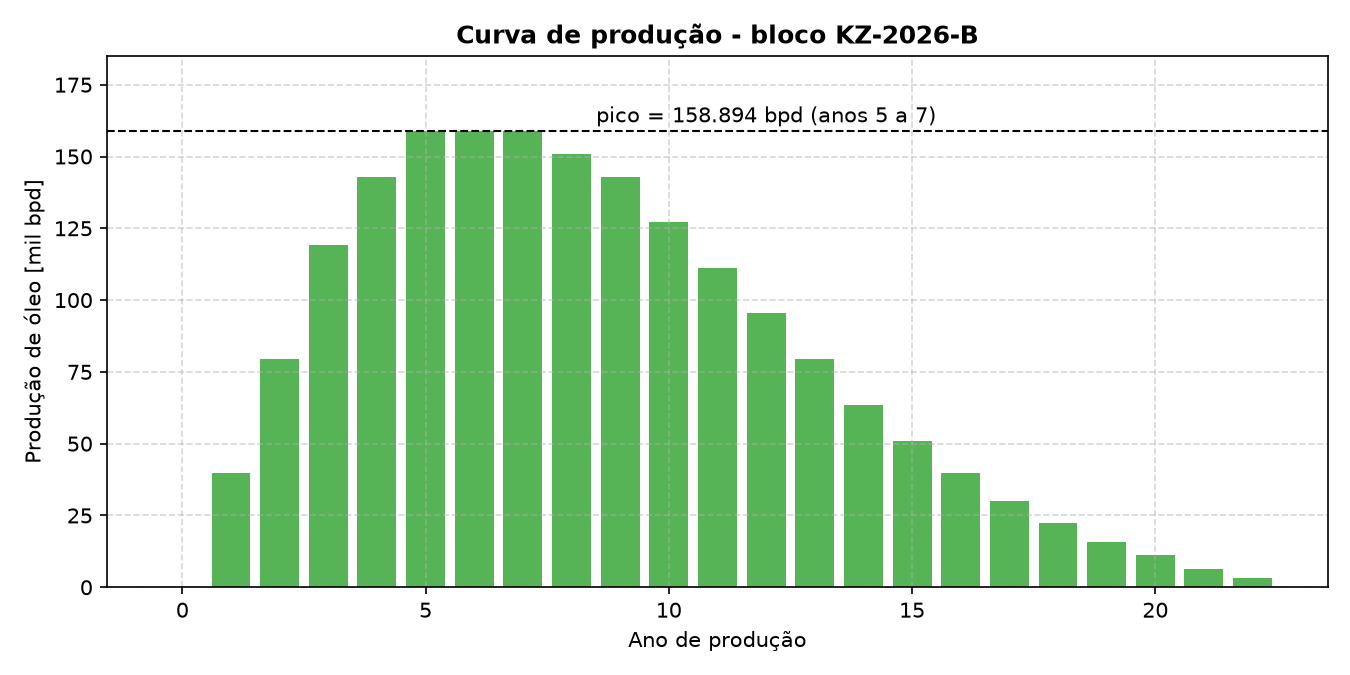
\includegraphics[width=\textwidth]{06_curva_producao.png}
\end{columns}
\end{frame}

\begin{frame}{Dados fixos e hipóteses de entrada}
\begin{columns}[T]
\column{0.5\textwidth}
\small
\begin{tabular}{lr}
\toprule
Dado & Valor \\
\midrule
BOE (só óleo) & 158.894 boe/dia \\
$\gamma_e$ & 0,270 t/m$^3$ \\
$h_d$ / $h_m$ (estimados) & 8 / 12 m \\
Vento tempestade / operação & 51,5 / 36 m/s \\
$H_s$, $T_p$ & 5,6 m, 15,2 s \\
$\xi$ & 0,05 \\
JONSWAP $\gamma$ & 3,3 \\
\bottomrule
\end{tabular}
\column{0.5\textwidth}
\small
\begin{itemize}
\item Vento de 100 anos do local é 24 m/s: o critério com 51,5 m/s é conservador (22\% do momento)
\item Planta dimensionada pelo pico de óleo; o caso com gás está na sensibilidade
\item $h_d$ e $h_m$ estimados: efeito quantificado na sensibilidade
\end{itemize}
\end{columns}
\end{frame}

% =============================================================================
\section{Modelo paramétrico}

\begin{frame}{Geometria e variáveis de projeto}
\begin{columns}[c]
\column{0.58\textwidth}
\centering
\begin{tikzpicture}[scale=0.32,>=Stealth]
  \begin{scope}
    \draw[thick] (-5,-5) rectangle (5,5);
    \fill[blue!25] (-5,3.6) rectangle (5,5);   \draw (-5,3.6) rectangle (5,5);
    \fill[blue!25] (-5,-5) rectangle (5,-3.6); \draw (-5,-5) rectangle (5,-3.6);
    \foreach \x in {-5,3.8} \foreach \y in {3.7,-4.9}
      \fill[green!50!black,opacity=.7] (\x,\y) rectangle ++(1.2,1.2);
    \draw[<->] (-5,-6) -- node[below]{$L_p$} (5,-6);
    \draw[<->] (5.6,3.6) -- node[right]{$b_p$} (5.6,5);
    \draw[<->] (-5,5.6) -- node[above]{$b_c$} (-3.8,5.6);
    \node at (0,-8.3) {\scriptsize Planta};
  \end{scope}
  \begin{scope}[xshift=15cm,yshift=-4cm]
    \fill[blue!25] (-5,0) rectangle (5,1.5); \draw (-5,0) rectangle (5,1.5);
    \fill[green!50!black,opacity=.7] (-5,1.5) rectangle (-3.8,6.5);
    \fill[green!50!black,opacity=.7] (3.8,1.5) rectangle (5,6.5);
    \fill[gray!60] (-5,6.5) rectangle (5,7.5);
    \fill[gray!25] (-5,7.5) rectangle (5,9);
    \draw[dashed,blue,thick] (-6.5,3.4) -- (6.5,3.4);
    \draw[<->] (-5.8,0) -- node[left]{$h_p$} (-5.8,1.5);
    \draw[<->] (-5.8,1.5) -- node[left]{$h_c$} (-5.8,6.5);
    \draw[<->] (6.9,0) -- node[right]{$T$} (6.9,3.4);
    \draw[<->] (0,3.4) -- node[right]{$a$} (0,6.5);
    \node at (0,-4.3) {\scriptsize Vista lateral};
  \end{scope}
\end{tikzpicture}
\column{0.42\textwidth}
\small
\begin{itemize}
\item 2 \emph{pontoons} retangulares, 4 colunas quadradas, planta quadrada
\item Variáveis: $x = (L_p, b_p, h_p, b_c, h_c, T)$
\item Objetivos: $\min W_{casco}$ e $\min \Hz$
\item Uma avaliação completa: $\approx$ 6 ms
\end{itemize}
\end{columns}
\end{frame}

\begin{frame}{Fluxo de cálculo}
\centering
\begin{tikzpicture}[node distance=2.5mm and 5mm,
  box/.style={draw,rounded corners,fill=blue!6,minimum width=5cm,minimum height=6mm,
              align=center,font=\scriptsize},
  arr/.style={-Stealth,thick}]
  \node[box,fill=orange!15] (x) {Variáveis $x = (L_p, b_p, h_p, b_c, h_c, T)$};
  \node[box,below=of x] (h) {1. Hidrostática (Ex. 7): $\nabla$, $\Delta$, KB, BM, KM};
  \node[box,below=of h] (p) {2. Pesos e centros (Ex. 8): $W_{casco}$, lastro, KG, GM};
  \node[box,below=of p] (c) {3. Convés e \emph{air gap} (Ex. 8): $L_p^2$, $a$};
  \node[box,below=of c] (g) {4. Curva GZ 2D (Ex. 9), $\phial$};
  \node[box,below=of g] (v) {5. Vento (Ex. 9): $HM_0$, $HM_{ud}$, $A/B$};
  \node[box,right=12mm of h] (f) {6. \emph{Heave} (Ex. 10): $F_3$, $A_{33}$, $T_n$, RAO};
  \node[box,below=of f] (s) {7. Espectro (Ex. 10): $S_z$, $\Hz$};
  \node[box,below=of s] (ag) {8. \emph{Air gap} mínimo: $\eta_{max}$, $z_{min}$, $\amin$};
  \node[box,below=of ag,fill=red!10] (r) {Restrições e objetivos};
  \node[box,below=of r,fill=green!12] (o) {LHS + soma ponderada + $\varepsilon$-restrito $\to$ Pareto};
  \draw[arr] (x)--(h); \draw[arr] (h)--(p); \draw[arr] (p)--(c); \draw[arr] (c)--(g);
  \draw[arr] (g)--(v); \draw[arr] (h.east)--(f.west); \draw[arr] (f)--(s); \draw[arr] (s)--(ag);
  \draw[arr] (ag)--(r); \draw[arr] (v.east)--(r.west); \draw[arr] (r)--(o);
\end{tikzpicture}
\end{frame}

\begin{frame}{Hidrostática, pesos e estabilidade}
\begin{columns}[T]
\column{0.5\textwidth}
\textbf{Hidrostática}
\small
\[
\nabla = 2L_pb_ph_p + 4b_c^2(T-h_p), \quad \Delta = \rho\nabla
\]
\[
I_T = 4\left(\tfrac{b_c^4}{12} + b_c^2 y_c^2\right),\quad BM = I/\nabla
\]
\textbf{Pesos}
\begin{itemize}
\item Planta: 0,083 t/boe; convés e operação: 35\% cada
\item Casco: $\gamma_e(2L_pb_ph_p + 4b_c^2h_c)$
\item \emph{Risers} 4\% $\Delta$, amarração 3\% $\Delta$
\item Lastro $= \Delta - \sum W$, no nível real de enchimento
\end{itemize}
\column{0.5\textwidth}
\textbf{GZ por projeções 2D}
\small
\begin{itemize}
\item Retângulos com espessura fora do plano, em cada plano
\item Linha d'água $z = \alpha + u\tan\varphi$ com $V(\alpha) = \nabla$ (Newton + bissecção)
\end{itemize}
\[
GZ = u_B\cos\varphi + (z_B - KG)\sin\varphi
\]
\textbf{Vento}
\begin{itemize}
\item 4 colunas sem sombra, \emph{deck box}, módulos, face inferior ($L_p^2$)
\item Braço até o $z_{CLR}$ de cada plano
\end{itemize}
\[
HA = \frac{HM_0\cos\varphi + HM_{ud}\sin\varphi}{\Delta g},\quad \frac{A}{B} \ge 1{,}3
\]
\end{columns}
\end{frame}

\begin{frame}{\emph{Heave} e \emph{air gap}}
\small
\[
A_{33} = 2(L_p - 2b_c)\,C_A\,\rho\pi\left(\tfrac{b_p}{2}\right)^2, \quad
C_{33} = \rho g\, 4b_c^2, \quad T_n = 2\pi\sqrt{\tfrac{\Delta + A_{33}}{C_{33}}}
\]
\[
\frac{F_3}{\zeta_a} = \cos\!\left(\tfrac{\omega^2 d_p}{2g}\right)\!\left[\rho g A_{wp}e^{-k(T-h_p)}
- \rho g A_p\left(e^{-k(T-h_p)} - e^{-kT}\right) - A_{33}\omega^2 e^{-k(T-h_p/2)}\right]
\]
\[
RAO = \frac{|F_3/\zeta_a|}{|C_{33} - (\Delta + A_{33})\omega^2 + iB_{33}\omega|}, \qquad
S_z = RAO^2 S_\zeta^{\text{JONSWAP}}, \qquad \Hz = 4\sqrt{m_{0z}}
\]
\[
\amin = \frac{1{,}86\,H_s}{2} + \frac{1{,}86\,\Hz}{2}, \qquad a = h_p + h_c - T \ge \amin
\]
\vspace{2mm}
\begin{block}{Restrições}
$L_p^2 \ge 11.563$ m$^2$ \quad $1 \le GM_T \le 4$ m \quad $T_n > 20$ s \quad
$0 < V_{lastro} \le 0{,}9V_{pont}$ \quad $b_c \le b_p$ \quad $A/B \ge 1{,}3$ (4 casos) \quad
$a \ge \amin$
\end{block}
\end{frame}

% =============================================================================
\section{Validação}

\begin{frame}{Validação: plataforma dos Exercícios 7 a 10}
\begin{columns}[c]
\column{0.42\textwidth}
\small
$L_p = 100$, $b_p = h_p = b_c = 15$, $h_c = 45$, $T = 30$ m; $H_s = 12{,}2$ m
\vspace{2mm}

\begin{tabular}{lrrr}
\toprule
 & Modelo & Aula & Erro \\
\midrule
KG [m] & 33,21 & 33,00 & 0,6\% \\
$A/B$ transv. & 2,31 & 2,33 & 0,9\% \\
$A/B$ long. & 2,27 & 2,36 & 3,7\% \\
$T_n$ [s] & 20,70 & 20,70 & 0,0\% \\
$\Hz$ [m] & 2,98 & 2,98 & 0,1\% \\
$\eta_{max}$ [m] & 11,35 & 11,35 & 0,0\% \\
\bottomrule
\end{tabular}
\vspace{2mm}

\footnotesize Consistência: $dGZ/d\varphi(0) = GM$, $RAO(\omega\to0) = 1$, $\sum W = \Delta$
\column{0.58\textwidth}
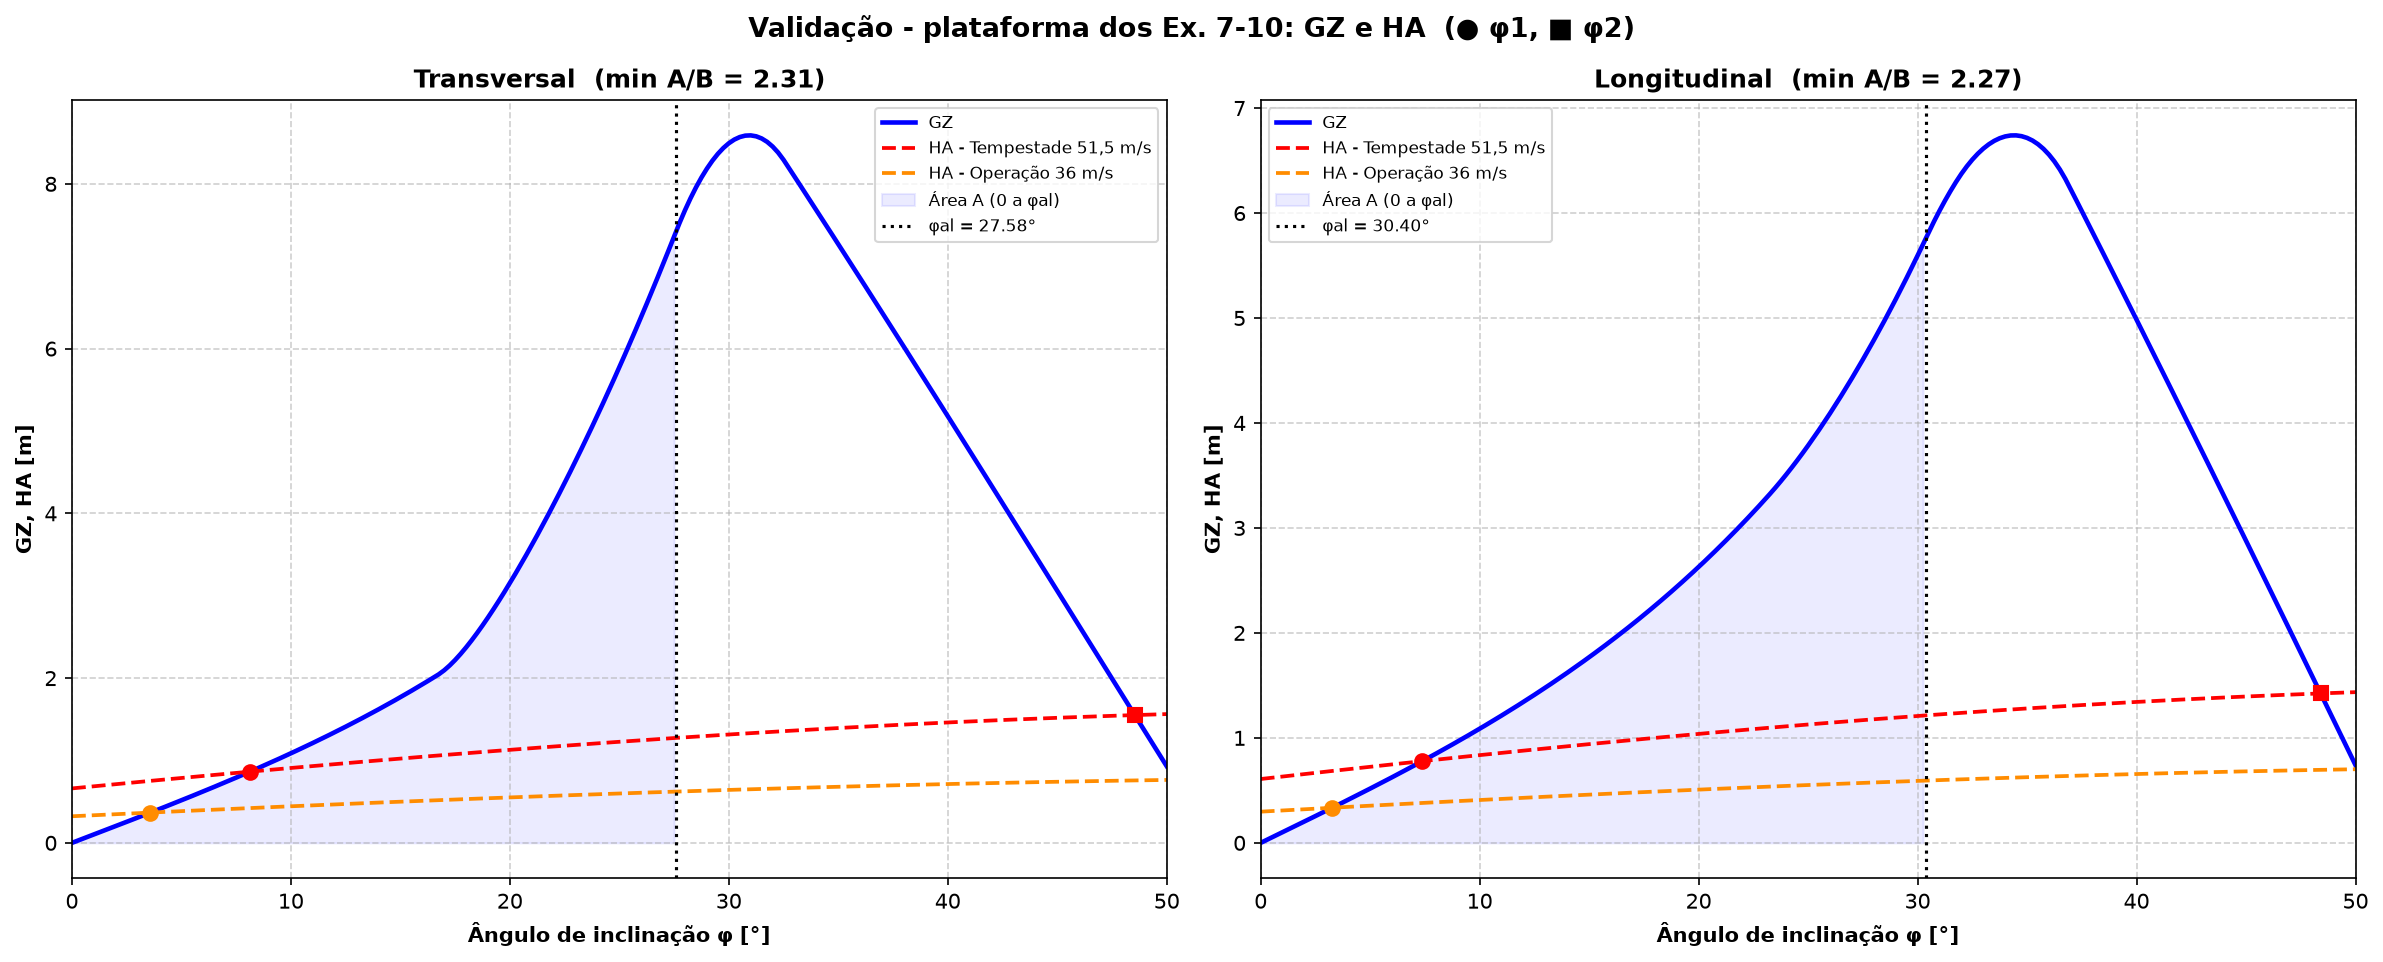
\includegraphics[width=\textwidth]{00_validacao_gz.png}
\end{columns}
\end{frame}

% =============================================================================
\section{Otimização e fronteira de Pareto}

\begin{frame}{Procedimento de variação sistemática}
\small
\begin{enumerate}
\item \textbf{Hipercubo latino:} 20.000 combinações no domínio
$107{,}5 \le L_p \le 150$, $8 \le b_p, b_c \le 25$, $6 \le h_p \le 20$, $20 \le h_c \le 50$,
$12 \le T \le 40$ m
\begin{itemize}
\item 547 atendem às restrições sem vento; só \textbf{227 (1,1\%)} passam no critério de áreas
\end{itemize}
\item \textbf{Soma ponderada} (SLSQP): $F = w_1\Hz + w_2 W_{casco}/10^4$,
$w_1 = 0; 0{,}05; \ldots; 1$
\begin{itemize}
\item 5 partidas do LHS + continuação do $w_1$ anterior, em paralelo
\item 7 dos 21 ótimos ficam dominados: a fronteira é não convexa
\end{itemize}
\item \textbf{$\varepsilon$-restrito:} $\min W_{casco}$ s.a. $\Hz \le \varepsilon$, 12 níveis
\item \textbf{Filtro de não dominância} sobre as 260 soluções viáveis $\Rightarrow$
\textbf{25 pontos}
\end{enumerate}
\vspace{1mm}
\footnotesize Na otimização a GZ usa passo de 1$^\circ$; todo ótimo é reconfirmado com
0,25$^\circ$. Rodada completa: $\approx$ 4 min em 8 núcleos.
\end{frame}

\begin{frame}{Conjunto viável e fronteira de Pareto}
\centering
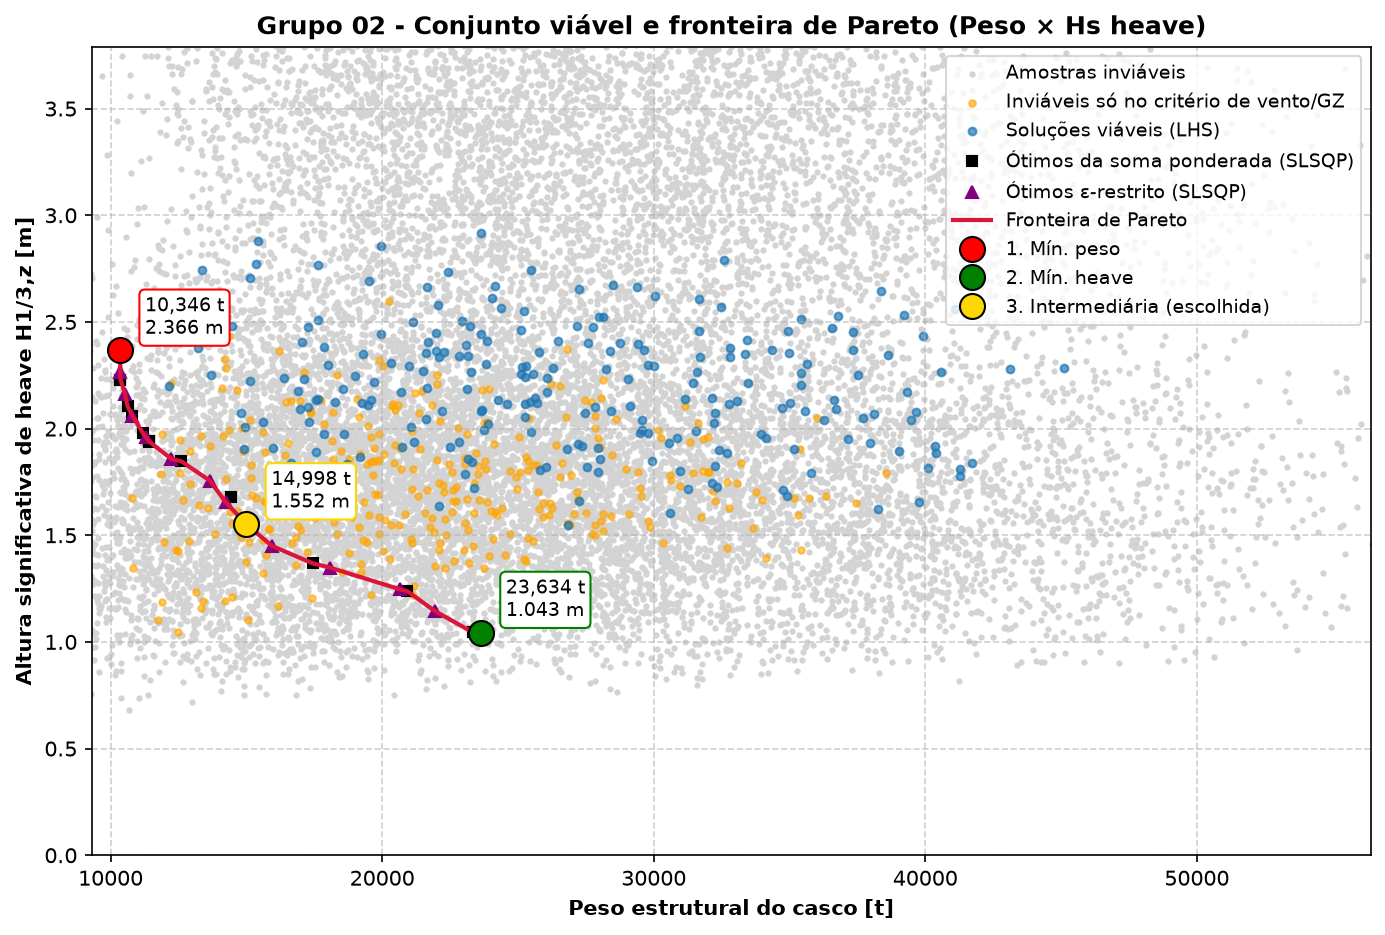
\includegraphics[height=0.86\textheight]{01_pareto.png}
\end{frame}

\begin{frame}{Restrições ativas e famílias de projeto}
\begin{columns}[T]
\column{0.38\textwidth}
\small
\textbf{Ativas nos 25 pontos:}
\begin{itemize}
\item $GM_T = 4$ m: 25
\item $A/B = 1{,}30$: 25
\item lastro $\approx 0$: 17
\item $b_c = b_p$: 9
\item área de convés: 4
\end{itemize}
\emph{Air gap} e $T_n$ nunca são ativos.
\vspace{2mm}

\textbf{Duas famílias:}
\begin{itemize}
\item rasa e larga ($L_p \to 150$ m, $T_n$ 29--40 s)
\item compacta e profunda ($L_p \approx 108$--118 m, $T_n \approx 22$ s)
\end{itemize}
\column{0.62\textwidth}
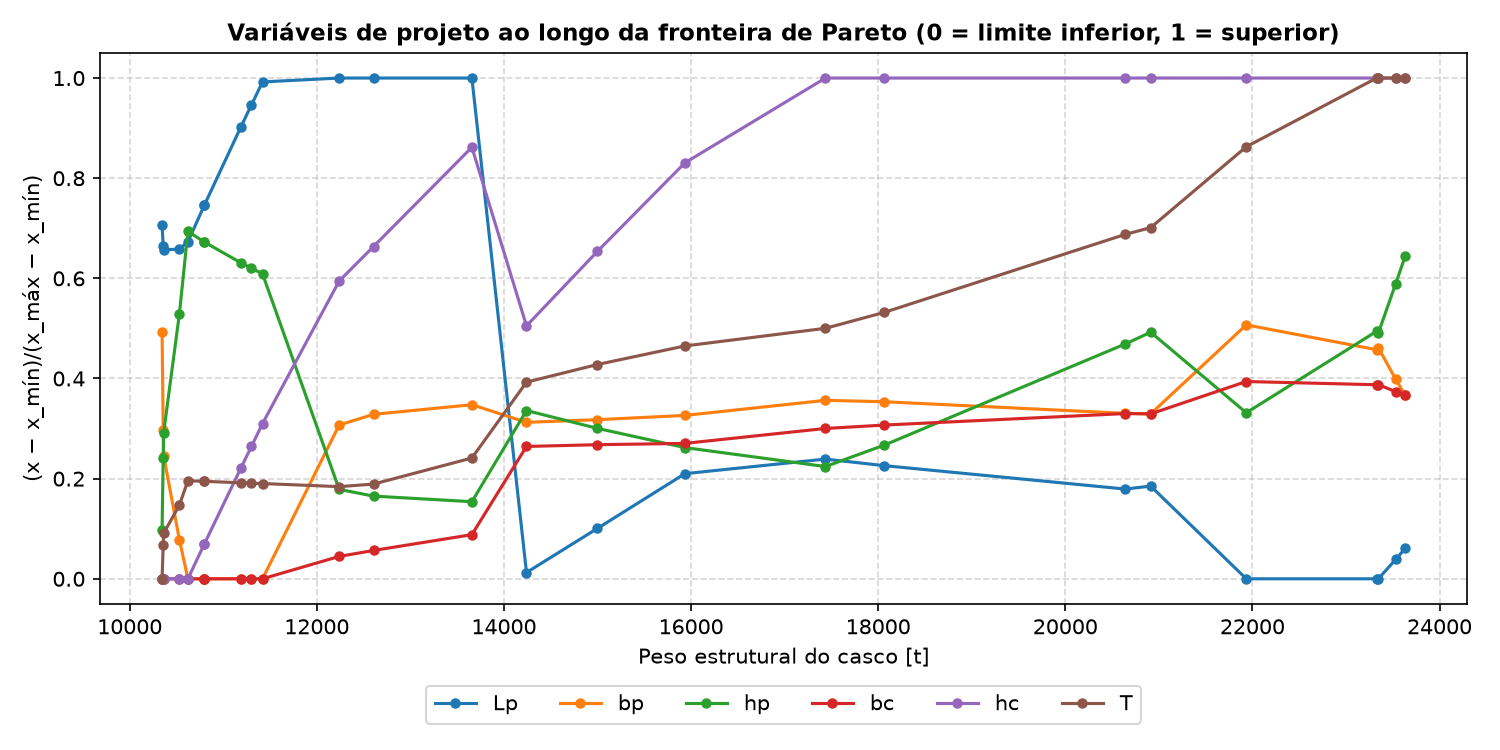
\includegraphics[width=\textwidth]{07_variaveis_fronteira.png}
\end{columns}
\end{frame}

% =============================================================================
\section{Os três cenários}

\begin{frame}{Ficha técnica comparativa}
\centering
\scriptsize
\begin{tabular}{lrrr}
\toprule
 & 1. Mín. peso & 2. Mín. \emph{heave} & 3. Intermediária \\
\midrule
$L_p$ / $b_p$ / $h_p$ [m] & 137,5 / 16,4 / 7,4 & 110,1 / 14,2 / 15,0 & 111,8 / 13,4 / 10,2 \\
$b_c$ / $h_c$ / $T$ [m] & 8,0 / 20,0 / 12,0 & 14,2 / 50,0 / 40,0 & 12,6 / 39,6 / 24,0 \\
Área de convés [m$^2$] & 18.905 & 12.125 & 12.499 \\
$\Delta$ [t] & 35.244 & 68.962 & 40.247 \\
\textbf{Peso do casco [t]} & \textbf{10.346} & \textbf{23.634} & \textbf{14.998} \\
Lastro [t] & 11 & 18.081 & 11 \\
KG / $GM_T$ / $GM_L$ [m] & 27,2 / 4,00 / 7,91 & 37,4 / 4,00 / 4,00 & 42,8 / 4,00 / 4,67 \\
$\phial$ transv. / long. [$^\circ$] & 9,0 / 9,8 & 24,4 / 24,4 & 21,6 / 23,9 \\
$\min A/B$ & 1,302 & 1,304 & 1,303 \\
$T_n$ [s] & 40,3 & 23,1 & 21,8 \\
\textbf{$\Hz$ [m]} & \textbf{2,366} & \textbf{1,043} & \textbf{1,552} \\
$\amin$ / $a$ [m] & 7,41 / 15,37 & 6,18 / 25,03 & 6,65 / 25,84 \\
Restrições ativas & $GM_T$, lastro, $A/B$ & $GM_T$, $b_c{=}b_p$, $A/B$ & $GM_T$, lastro, $A/B$ \\
Variáveis no limite & $b_c$, $h_c$, $T$ mín. & $h_c$, $T$ máx. & nenhuma \\
\bottomrule
\end{tabular}
\end{frame}

\begin{frame}{Vista lateral dos três cenários}
\centering
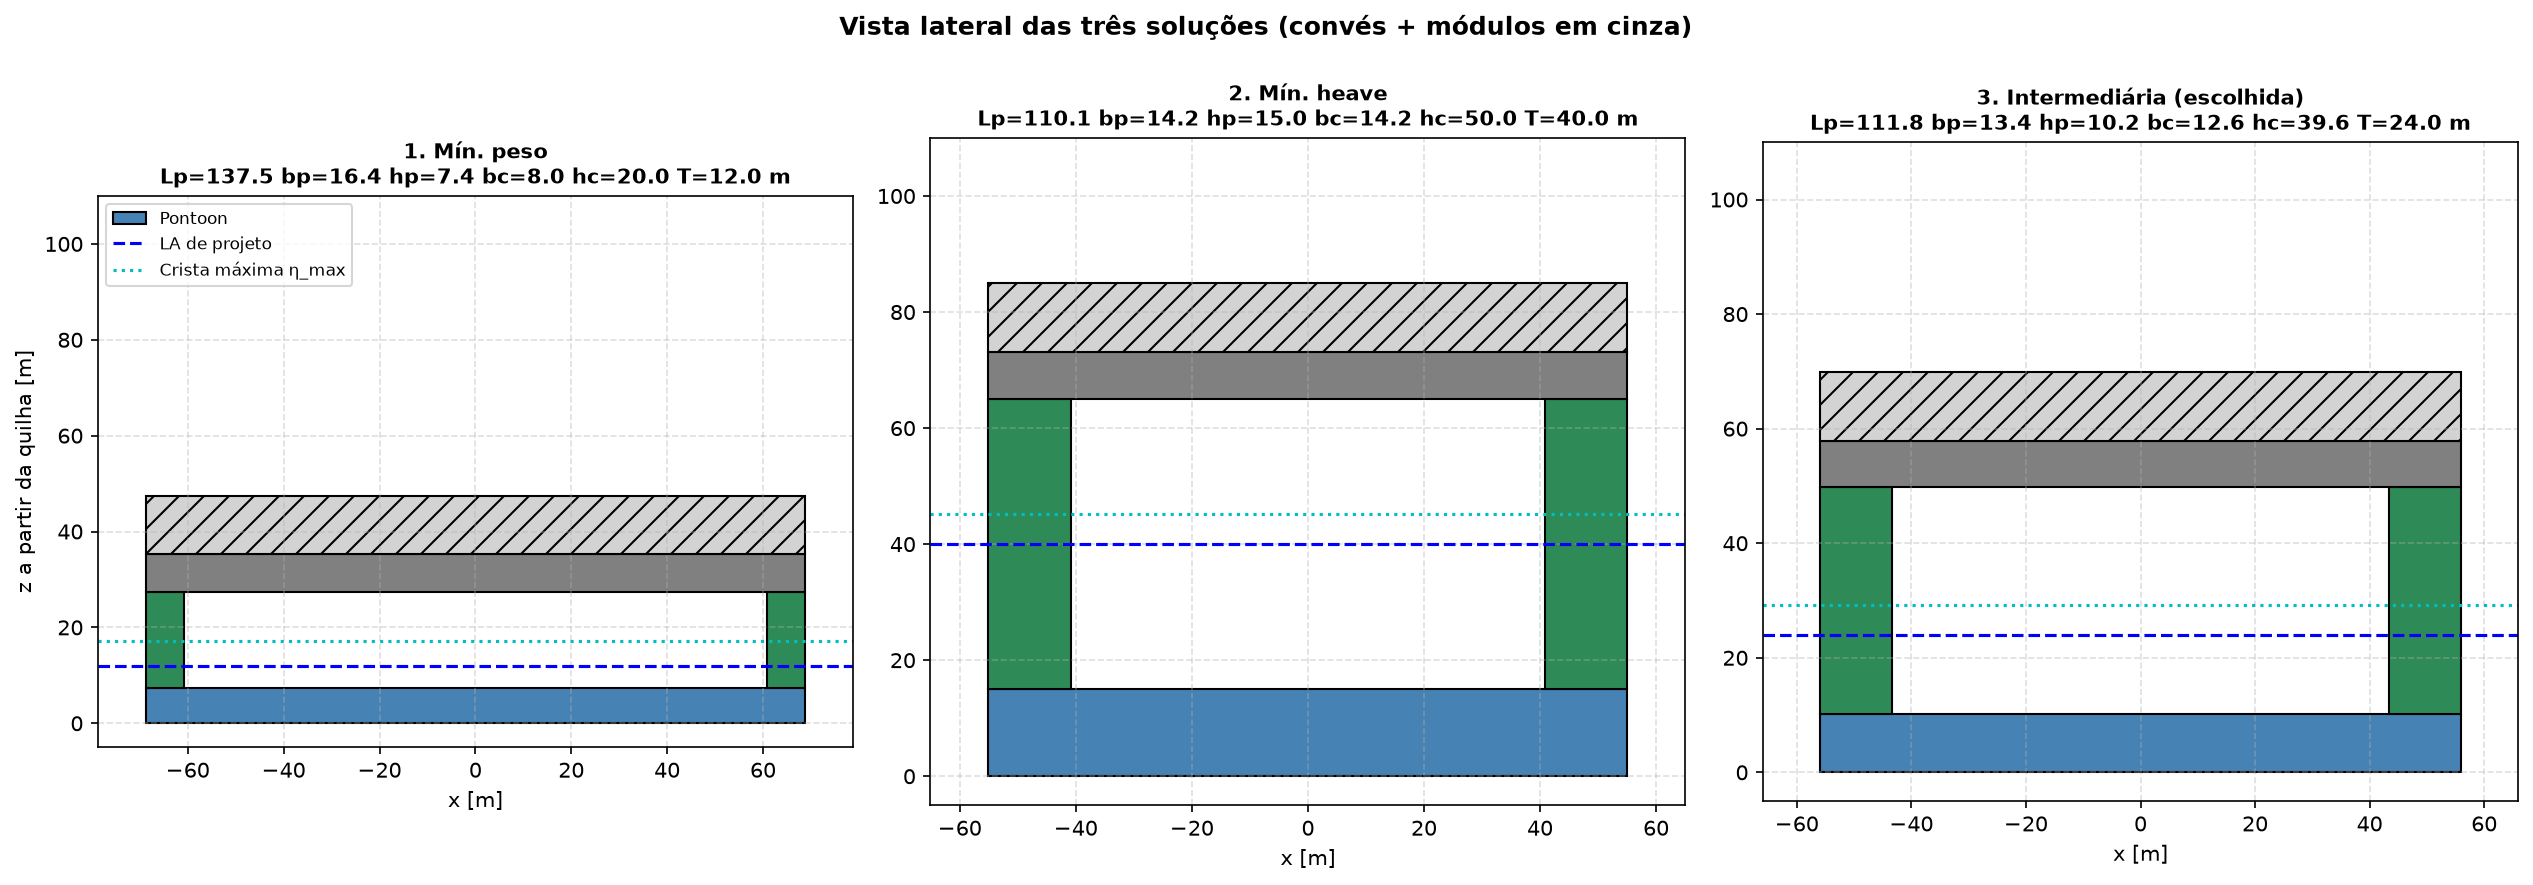
\includegraphics[width=\textwidth]{05_geometria_3_cenarios.png}
\end{frame}

\begin{frame}{Cenários extremos}
\begin{columns}[T]
\column{0.5\textwidth}
\textbf{1. Mínimo peso}
\scriptsize
\begin{itemize}
\item Semi rasa: $T$, $h_c$, $b_c$ no mínimo; \emph{pontoons} = 87\% do casco
\item Topo dos \emph{pontoons} a 4,6 m: $\Hz/H_s = 42\%$
\item $\phial = 9^\circ$, inclinação de 4,9$^\circ$ sob tempestade
\end{itemize}
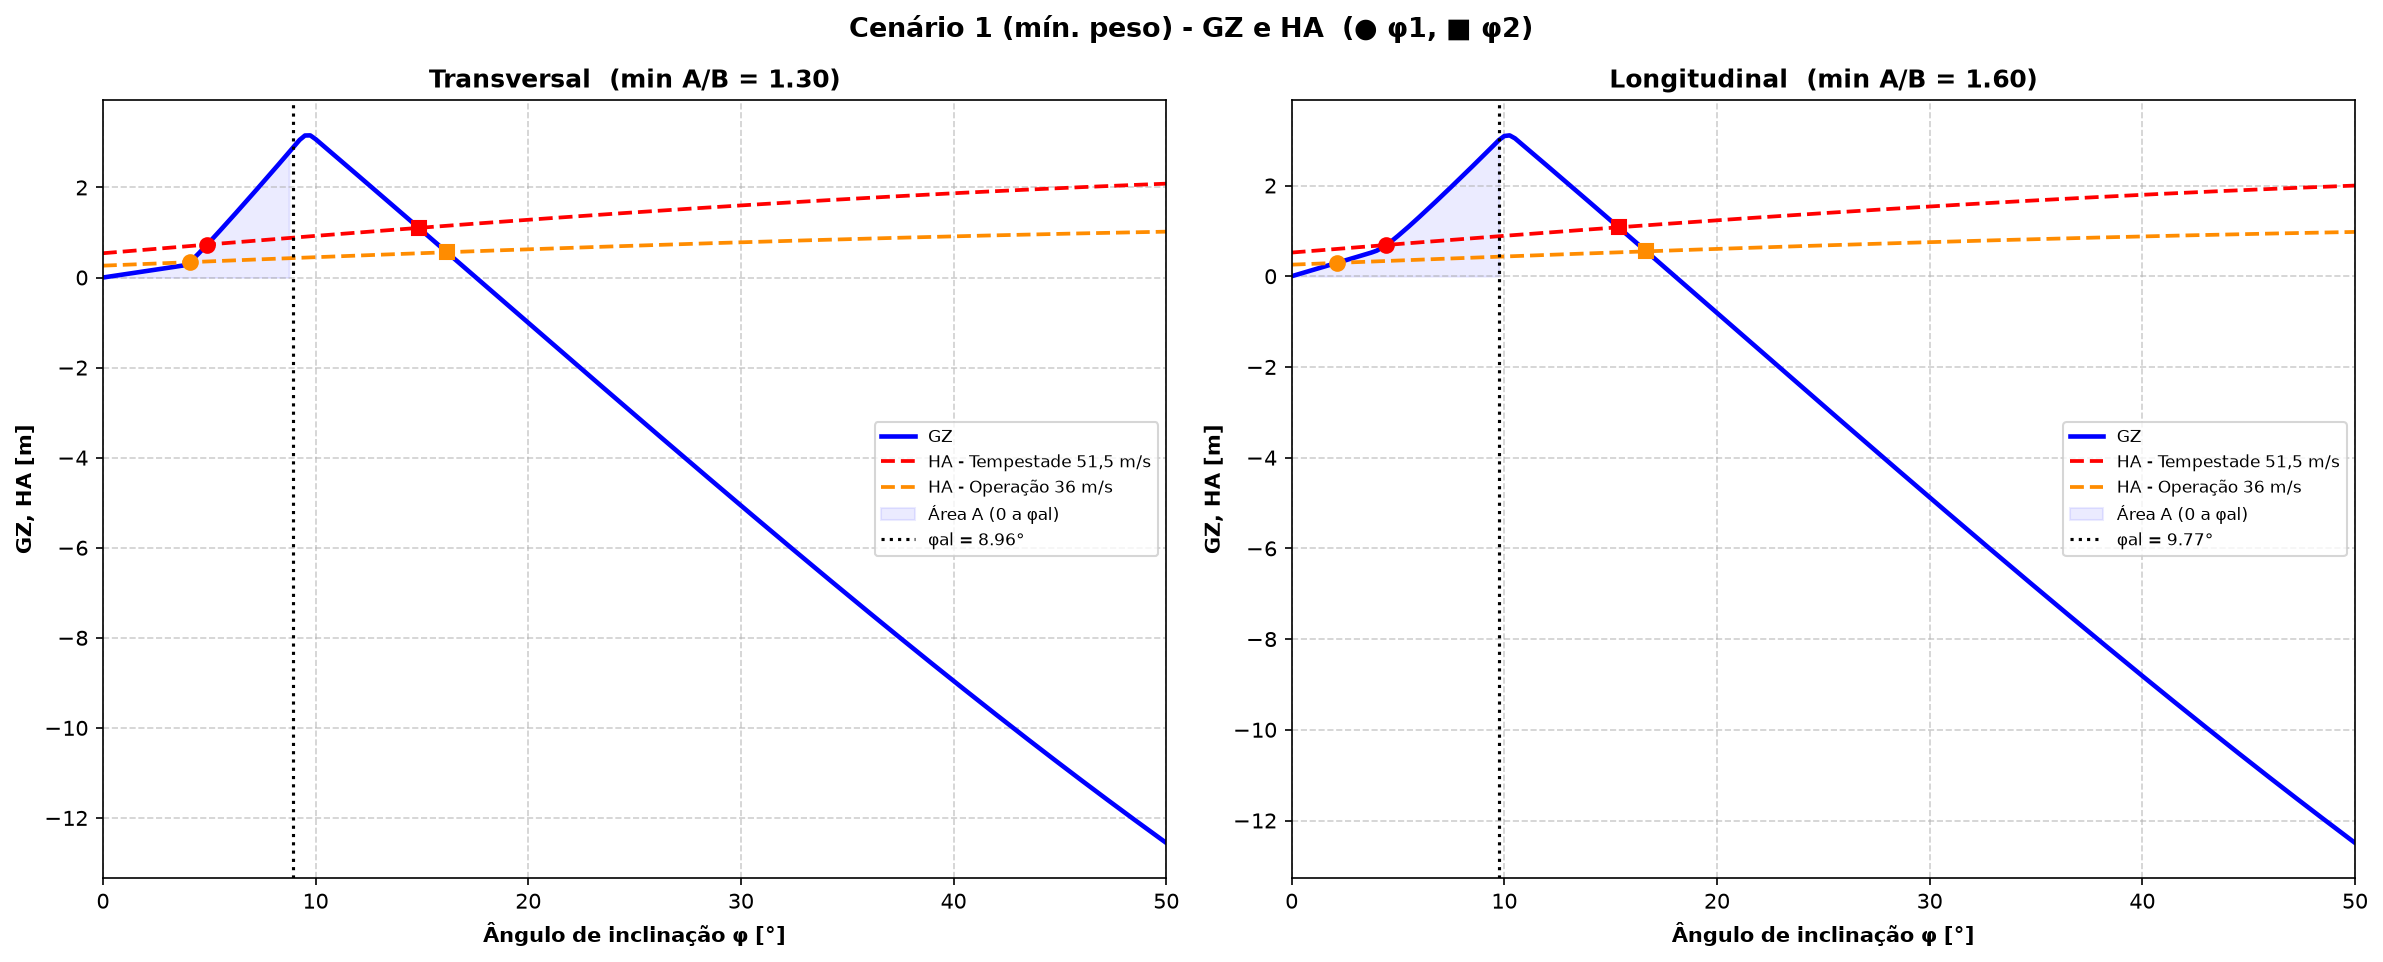
\includegraphics[width=\textwidth]{04a_gz_min_peso.png}
\column{0.5\textwidth}
\textbf{2. Mínimo \emph{heave}}
\scriptsize
\begin{itemize}
\item Calado profundo: $T = 40$, $h_c = 50$ m (máximos), $b_c = b_p$
\item $\Hz/H_s = 19\%$, único com lastro real (18.081 t)
\item Casco 2,3$\times$ mais pesado; fim da fronteira quase plano
\end{itemize}
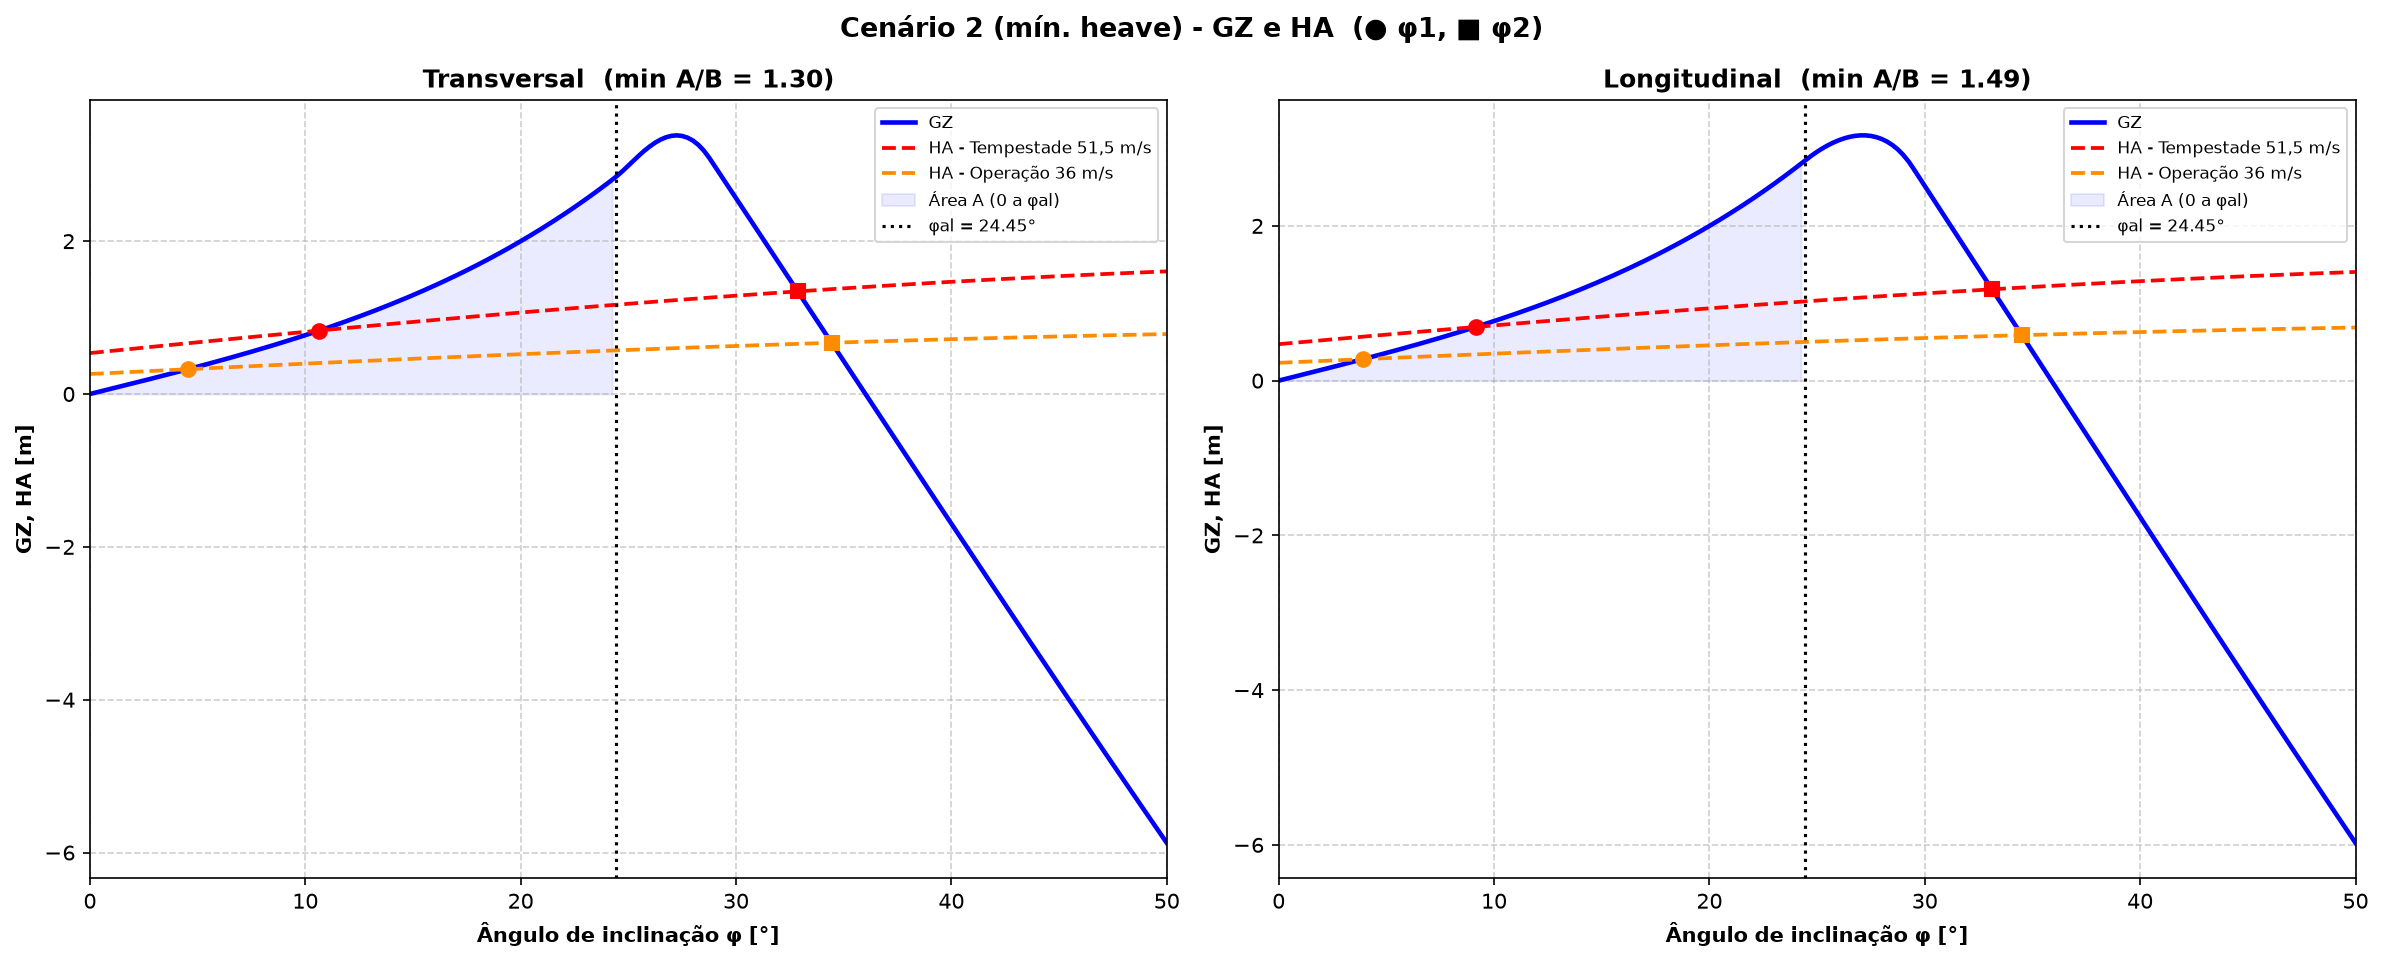
\includegraphics[width=\textwidth]{04b_gz_min_heave.png}
\end{columns}
\end{frame}

% =============================================================================
\section{Solução final}

\begin{frame}{Solução final: dimensões e pesos}
\begin{columns}[T]
\column{0.42\textwidth}
\small
\begin{tabular}{lr}
\toprule
$L_p$ & 111,80 m \\
$b_p$ / $h_p$ & 13,40 / 10,21 m \\
$b_c$ / $h_c$ & 12,55 / 39,61 m \\
$T$ & 23,98 m \\
Área de convés & 12.499 m$^2$ (+8\%) \\
$\Delta$ & 40.247 t \\
KB / KG & 7,75 / 42,82 m \\
$GM_T$ / $GM_L$ & 4,00 / 4,67 m \\
\bottomrule
\end{tabular}
\column{0.58\textwidth}
\scriptsize
\begin{tabular}{lrr}
\toprule
Item & Peso [t] & VCG [m] \\
\midrule
Planta de produção & 13.188 & 63,82 \\
Estrutura do convés & 4.616 & 53,82 \\
Carga operacional & 4.616 & 53,82 \\
\emph{Pontoons} & 8.257 & 5,10 \\
Colunas & 6.741 & 30,01 \\
\emph{Risers} + amarração & 2.817 & 49,82 \\
Lastro & 11 & 0,00 \\
\midrule
\textbf{Total} & \textbf{40.247} & \textbf{42,82} \\
\bottomrule
\end{tabular}
\end{columns}
\end{frame}

\begin{frame}{Solução final: GZ e braço de vento}
\centering
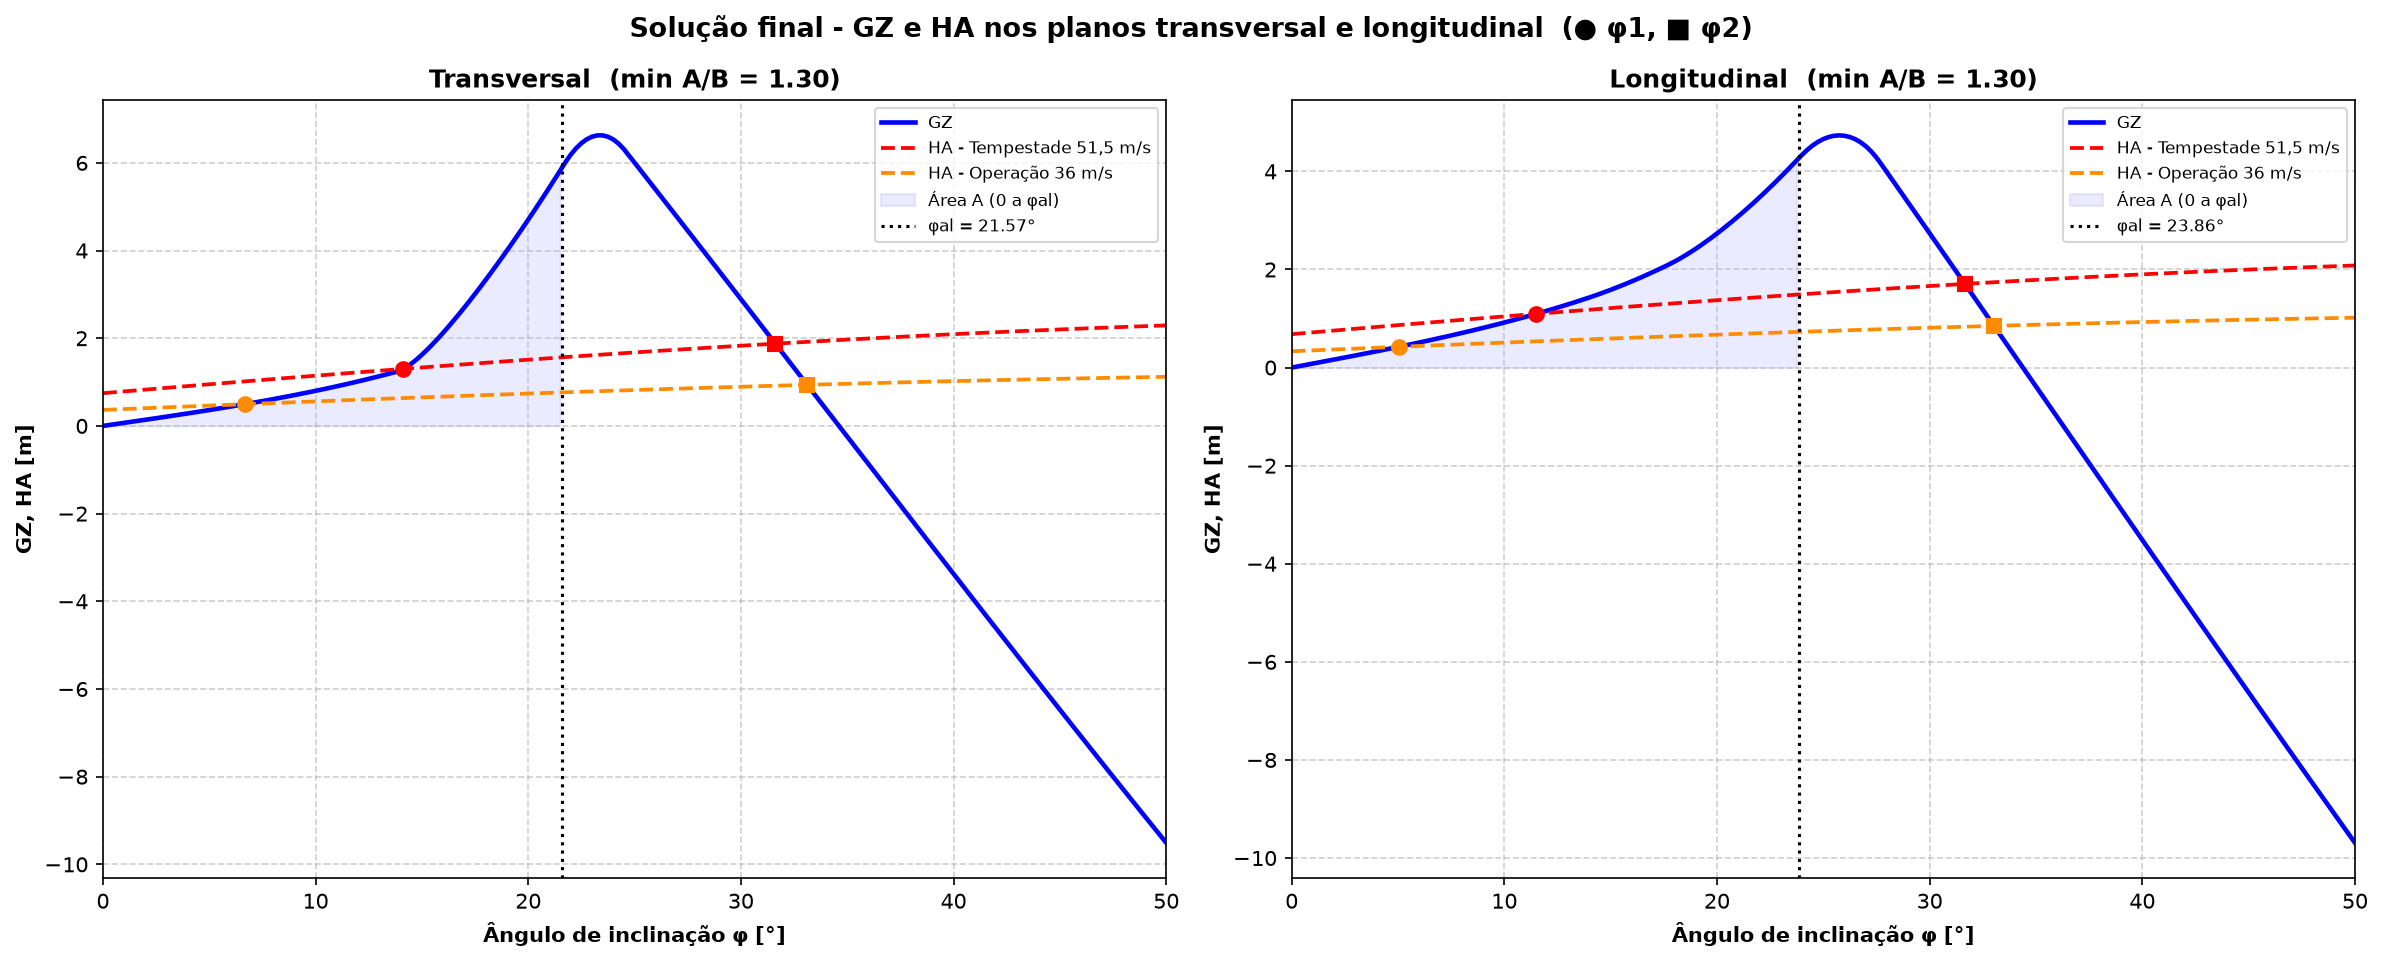
\includegraphics[width=\textwidth]{02_gz_ha_solucao_final.png}
\end{frame}

\begin{frame}{Solução final: vento e critério de áreas}
\scriptsize
\centering
\begin{tabular}{lrrrrrrrr}
\toprule
Parcela & Área [m$^2$] & $z$ [m] & $C_s$ & $C_h$ & $F_{51,5}$ [kN] & $F_{36}$ [kN] & Braço T [m] & Braço L [m] \\
\midrule
Colunas (4) & 1.297 & 12,9 & 1,0 & 1,00 & 2.102 & 1.027 & 29,0 & 25,1 \\
\emph{Deck box} & 894 & 29,8 & 1,0 & 1,10 & 1.594 & 779 & 45,9 & 42,0 \\
Módulos & 1.342 & 39,8 & 1,1 & 1,20 & 2.870 & 1.402 & 55,9 & 52,0 \\
Face inferior & 12.499 & 25,8 & 1,0 & 1,10 & 22.281 & 10.887 & 41,9 & 38,0 \\
\bottomrule
\end{tabular}
\vspace{3mm}

\begin{tabular}{llrrrrrrrr}
\toprule
Plano & Vento & $HM_0$ [kN$\cdot$m] & $HM_{ud}$ [kN$\cdot$m] & $\varphi_1$ & $\varphi_2$ & $\phial$ & $A$ & $B$ & $A/B$ \\
\midrule
Transv. & 51,5 m/s & 294.706 & 934.163 & 14,1$^\circ$ & 31,6$^\circ$ & 21,6$^\circ$ & 0,574 & 0,440 & \textbf{1,303} \\
Transv. & 36 m/s & 144.005 & 456.471 & 6,7$^\circ$ & 33,1$^\circ$ & 21,6$^\circ$ & 0,574 & 0,215 & 2,667 \\
Long. & 51,5 m/s & 269.057 & 847.134 & 11,5$^\circ$ & 31,7$^\circ$ & 23,9$^\circ$ & 0,598 & 0,459 & 1,304 \\
Long. & 36 m/s & 131.473 & 413.945 & 5,0$^\circ$ & 33,0$^\circ$ & 23,9$^\circ$ & 0,598 & 0,224 & 2,669 \\
\bottomrule
\end{tabular}
\vspace{3mm}

\small A face inferior do convés gera 3,2$\times$ o $HM_0$; o plano transversal é o crítico
($z_{CLR} = 7{,}9$ m contra 11,8 m).
\end{frame}

\begin{frame}{Solução final: \emph{heave}}
\begin{columns}[c]
\column{0.68\textwidth}
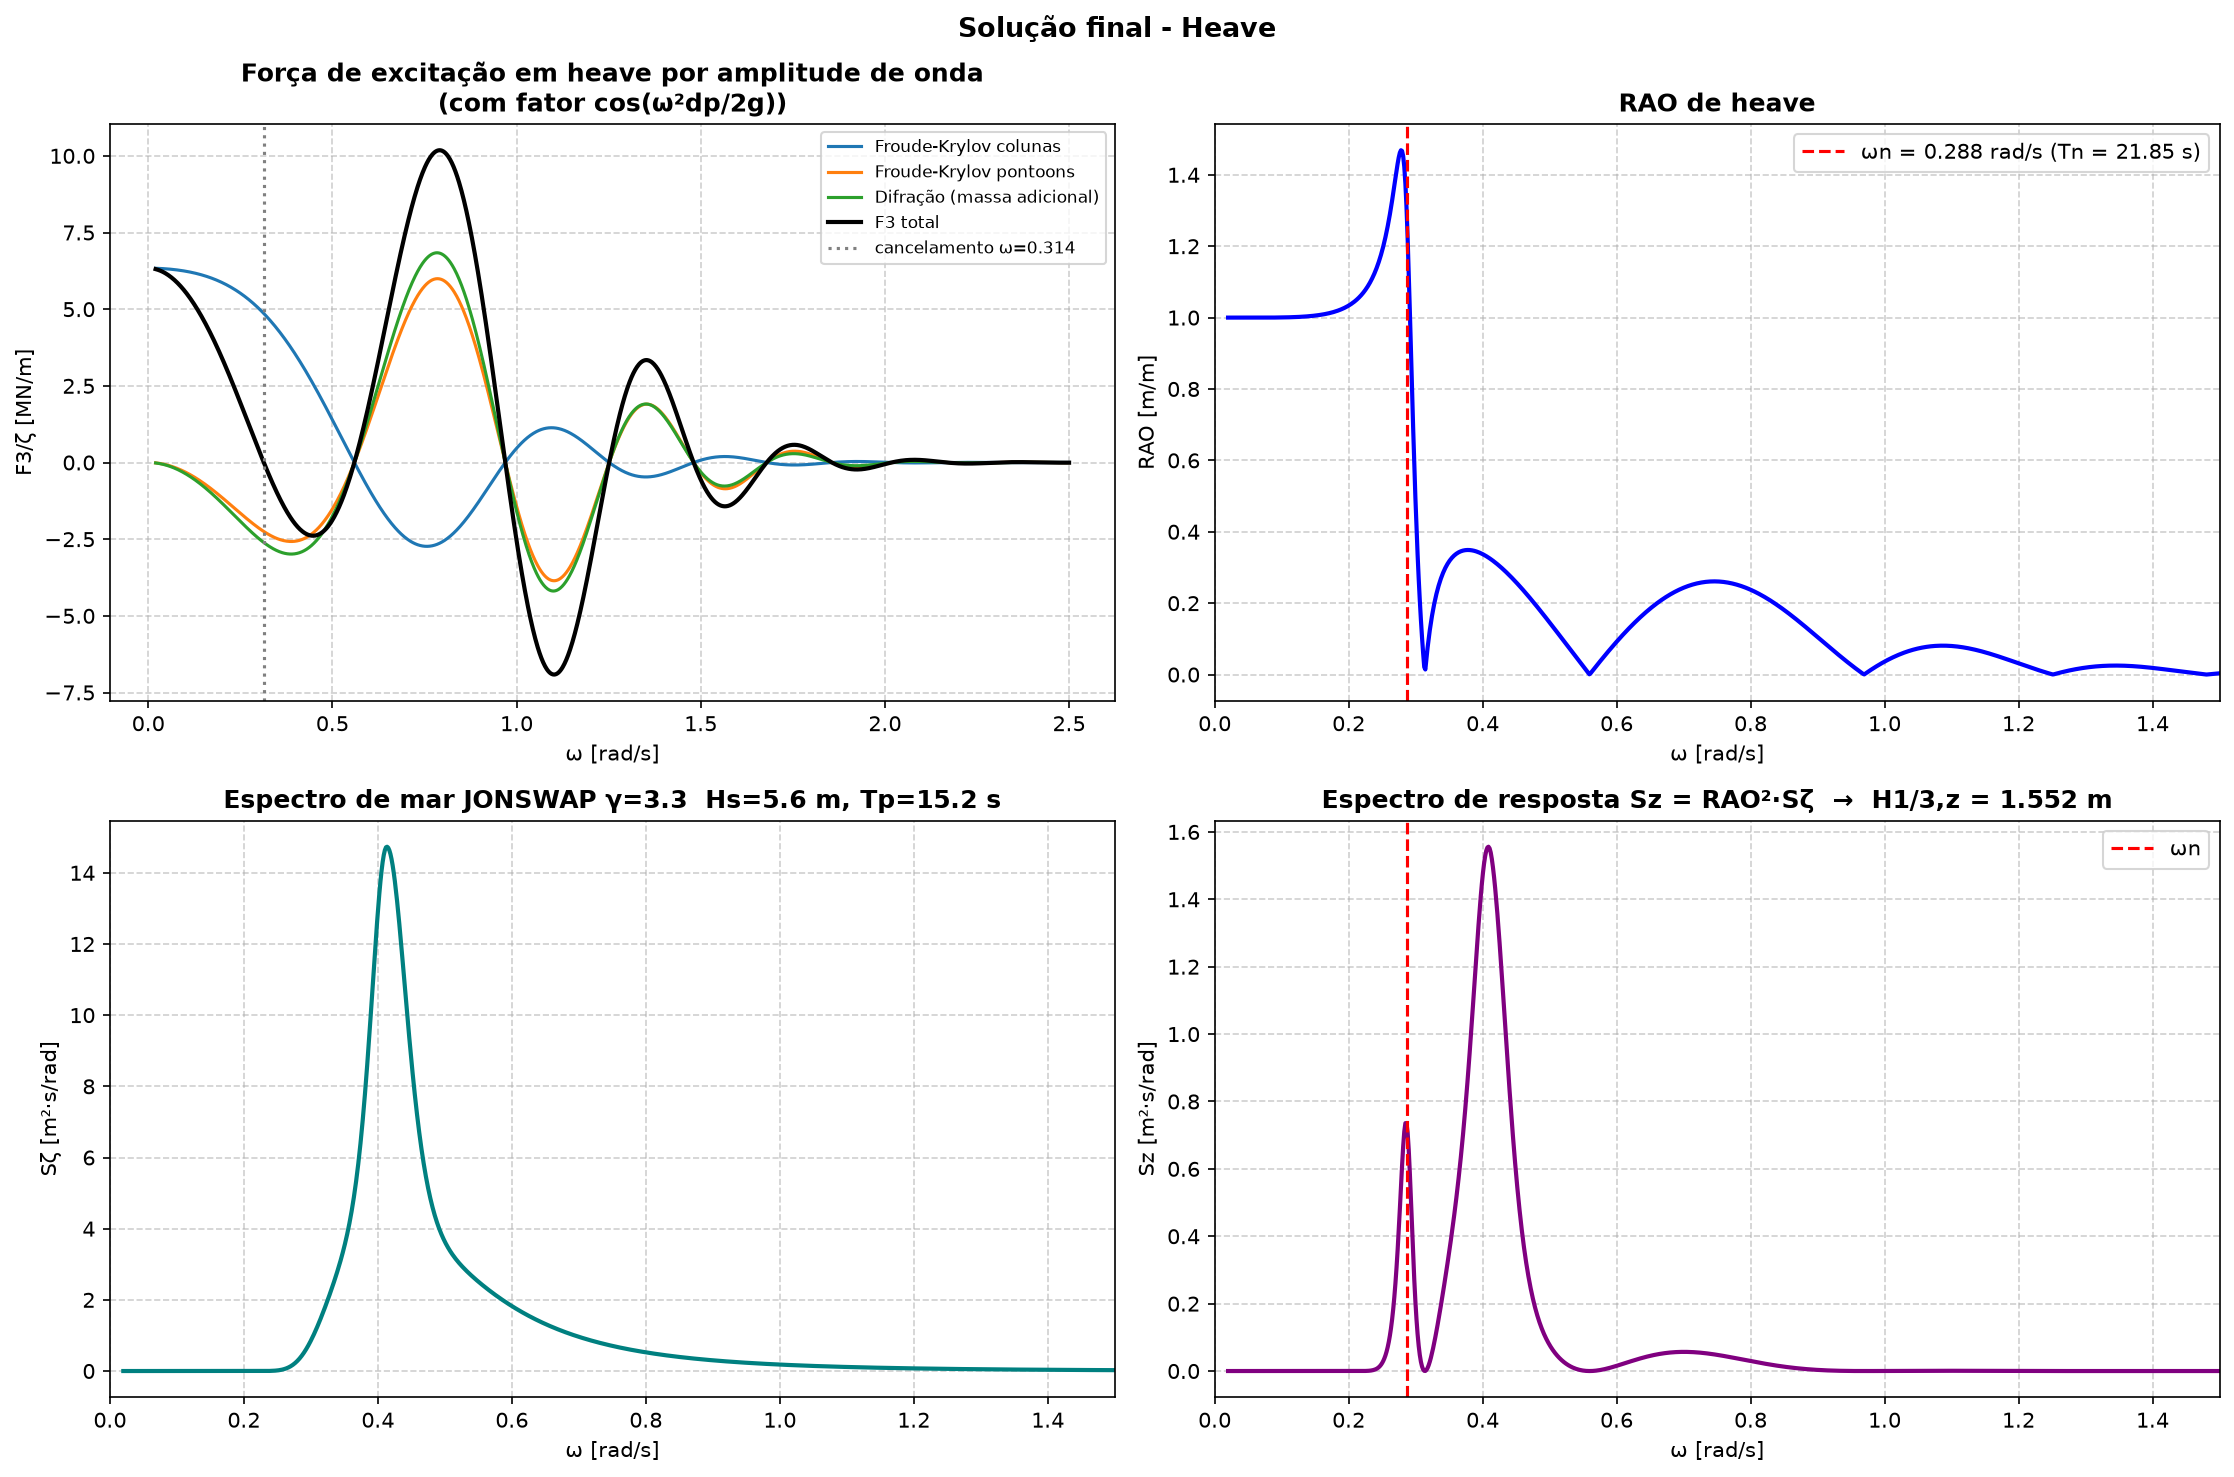
\includegraphics[width=\textwidth]{03_heave_solucao_final.png}
\column{0.32\textwidth}
\small
\begin{itemize}
\item $A_{33} = 36.378$ t, $C_{33} = 6.337$ kN/m
\item $T_n = 21{,}85$ s (9\% acima do limite)
\item Cancelamento da força em $\omega = 0{,}314$ rad/s, logo acima de $\omega_n = 0{,}288$:
pico do RAO limitado a 1,47
\item No pico do mar, RAO = 0,32
\item $\Hz = 1{,}552$ m ($\gamma = 3{,}3$); 1,454 m ($\gamma = 1$)
\end{itemize}
\end{columns}
\end{frame}

\begin{frame}{Solução final: \emph{air gap} e resumo das restrições}
\begin{columns}[T]
\column{0.34\textwidth}
\small
\begin{tabular}{lr}
\toprule
$\eta_{max}$ & 5,21 m \\
$z_{min}$ & $-1{,}44$ m \\
$\amin$ & 6,65 m \\
$a$ & 25,84 m \\
Folga & 19,19 m \\
\bottomrule
\end{tabular}
\vspace{2mm}

\footnotesize $h_c$ é definido pelo $\phial$ do critério de vento, não pela crista.
\column{0.66\textwidth}
\scriptsize
\begin{tabular}{lrrrl}
\toprule
Restrição & Valor & Limite & Folga & \\
\midrule
$L_p^2$ [m$^2$] & 12.499 & $\ge$ 11.563 & 8,1\% & \\
$GM_T$ [m] & 4,000 & $\le$ 4 & 0,0\% & \textbf{ativa} \\
$T_n$ [s] & 21,85 & $>$ 20 & 9,2\% & \\
Lastro [t] & 11 & $>$ 0 & -- & \textbf{ativa} \\
$V_{lastro}/V_{pont}$ & 0,000 & $\le$ 0,9 & -- & \\
$b_c$ [m] & 12,55 & $\le$ 13,40 & 6,3\% & \\
$a$ [m] & 25,84 & $\ge$ 6,65 & 288\% & \\
$\min A/B$ & 1,303 & $\ge$ 1,3 & 0,2\% & \textbf{ativa} \\
$GZ > 0$ até $\phial$ & sim & -- & -- & \\
\bottomrule
\end{tabular}
\end{columns}
\end{frame}

\begin{frame}{Por que a solução intermediária}
\begin{columns}[T]
\column{0.5\textwidth}
\small
\begin{itemize}
\item Joelho da fronteira: ponto mais próximo do utópico no plano normalizado
\item Contra o cenário 1: +45\% de peso, $-34$\% de $\Hz$
\item Contra o cenário 2: $-37$\% de peso, +49\% de $\Hz$
\item Única com todas as variáveis no interior do domínio
\item $\phial = 21{,}6^\circ$ contra 9,0$^\circ$ do cenário 1
\end{itemize}
\column{0.5\textwidth}
\small
\begin{block}{Custo marginal de reduzir o \emph{heave}}
\begin{tabular}{lrr}
\toprule
Trecho & $\Delta W$ [t] & t por mm \\
\midrule
1 $\to$ 3 & 4.652 & 5,7 \\
3 $\to$ 2 & 8.635 & 17,0 \\
\bottomrule
\end{tabular}
\end{block}
Depois do joelho, cada milímetro de \emph{heave} custa 3$\times$ mais peso.
\end{columns}
\end{frame}

% =============================================================================
\section{Sensibilidade e conclusões}

\begin{frame}{Análise de sensibilidade}
\begin{columns}[T]
\column{0.52\textwidth}
\scriptsize
\textbf{Reotimizações (solução intermediária):}
\vspace{1mm}

\begin{tabular}{lrrr}
\toprule
Caso & $W_{casco}$ [t] & Var. & $\Hz$ [m] \\
\midrule
Caso-base & 14.998 & -- & 1,552 \\
$h_m = 15$ m & 15.792 & +5,3\% & 1,560 \\
Com gás (203 mil boe/d) & 18.718 & +24,8\% & 1,373 \\
Lastro $\ge$ 10\% & 16.026 & +6,9\% & 1,549 \\
\bottomrule
\end{tabular}
\vspace{2mm}

\begin{itemize}
\item Geometria fixa: só é viável com $h_d = 8$ e $h_m = 12$ m (solução ajustada a $GM_T$ e $A/B$)
\item $\Hz$: 7\% com $\gamma$, 12\% com $\xi$; efeito em $\amin$ $< 0{,}2$ m
\end{itemize}
\column{0.48\textwidth}
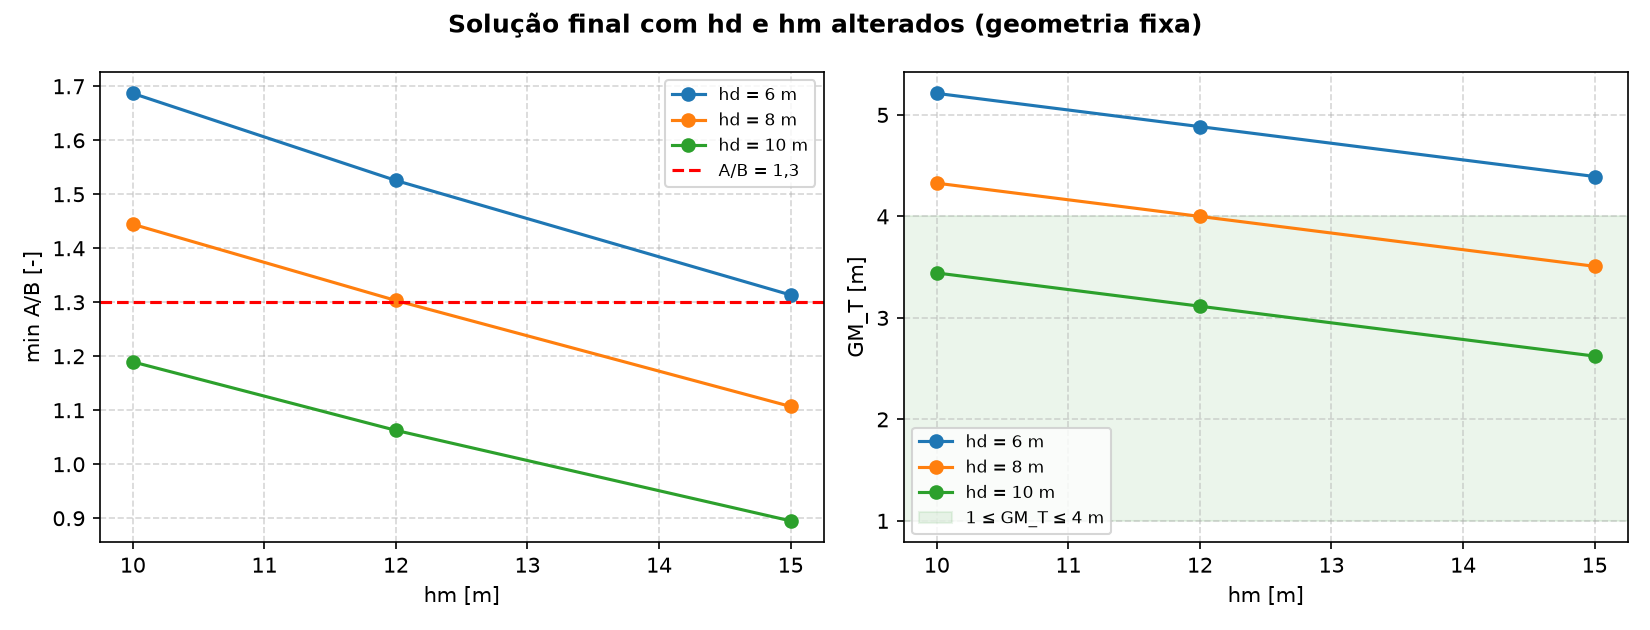
\includegraphics[width=\textwidth]{08_sensibilidade_hd_hm.png}
\end{columns}
\end{frame}

\begin{frame}{Conclusões}
\small
\begin{itemize}
\item O modelo cobre os 8 itens pedidos e reproduz as aulas com erro de até 3,7\%
\item Só 1,1\% do domínio é viável; o critério de áreas é a restrição mais seletiva
\item Fronteira de Pareto: 10.346 t ($\Hz = 2{,}37$ m) a 23.634 t ($\Hz = 1{,}04$ m)
\item O projeto é governado pela estabilidade: $GM_T = 4$ m e $A/B = 1{,}30$ ativos em todos os
ótimos
\item \textbf{Solução escolhida:} $L_p = 111{,}8$ m, $T = 24{,}0$ m, 14.998 t, $\Hz = 1{,}55$ m,
$T_n = 21{,}8$ s
\end{itemize}
\vspace{2mm}
\begin{block}{Próximos passos}
\small
Confirmar se o gás entra no BOE (+25\% no casco) $\cdot$ fundamentar $h_d$ e $h_m$ com o pôster
de semis $\cdot$ adotar lastro mínimo (+7\%) $\cdot$ validar com uma plataforma real $\cdot$
incluir roll/pitch no \emph{air gap}
\end{block}
\end{frame}

\begin{frame}
\centering
\vspace{1cm}
{\Huge Obrigado!}\\[6mm]
{\large Perguntas?}\\[10mm]
\small Código, resultados e relatório no repositório do grupo
\end{frame}

\end{document}
